\Aufgabe{SQL: Tabellen verbinden}{
    Wir kennen jetzt Tabellen, die miteinander über Fremd- und Primärschlüssel in Beziehung stehen. Nun möchten wir aus diesen Tabellen auch zusammengehörende Datensätze abfragen.

    Öffne dafür \UrlAndCode{www.dbiu.de/flugverspaetungen} und führe folgende SQL-Abfrage aus:

    \begin{center}
        \emphColB{
        SELECT *\\
        FROM Fluggesellschaft, Flug}
    \end{center}

}

\ifbeamer
\definesframe[false]{}{
    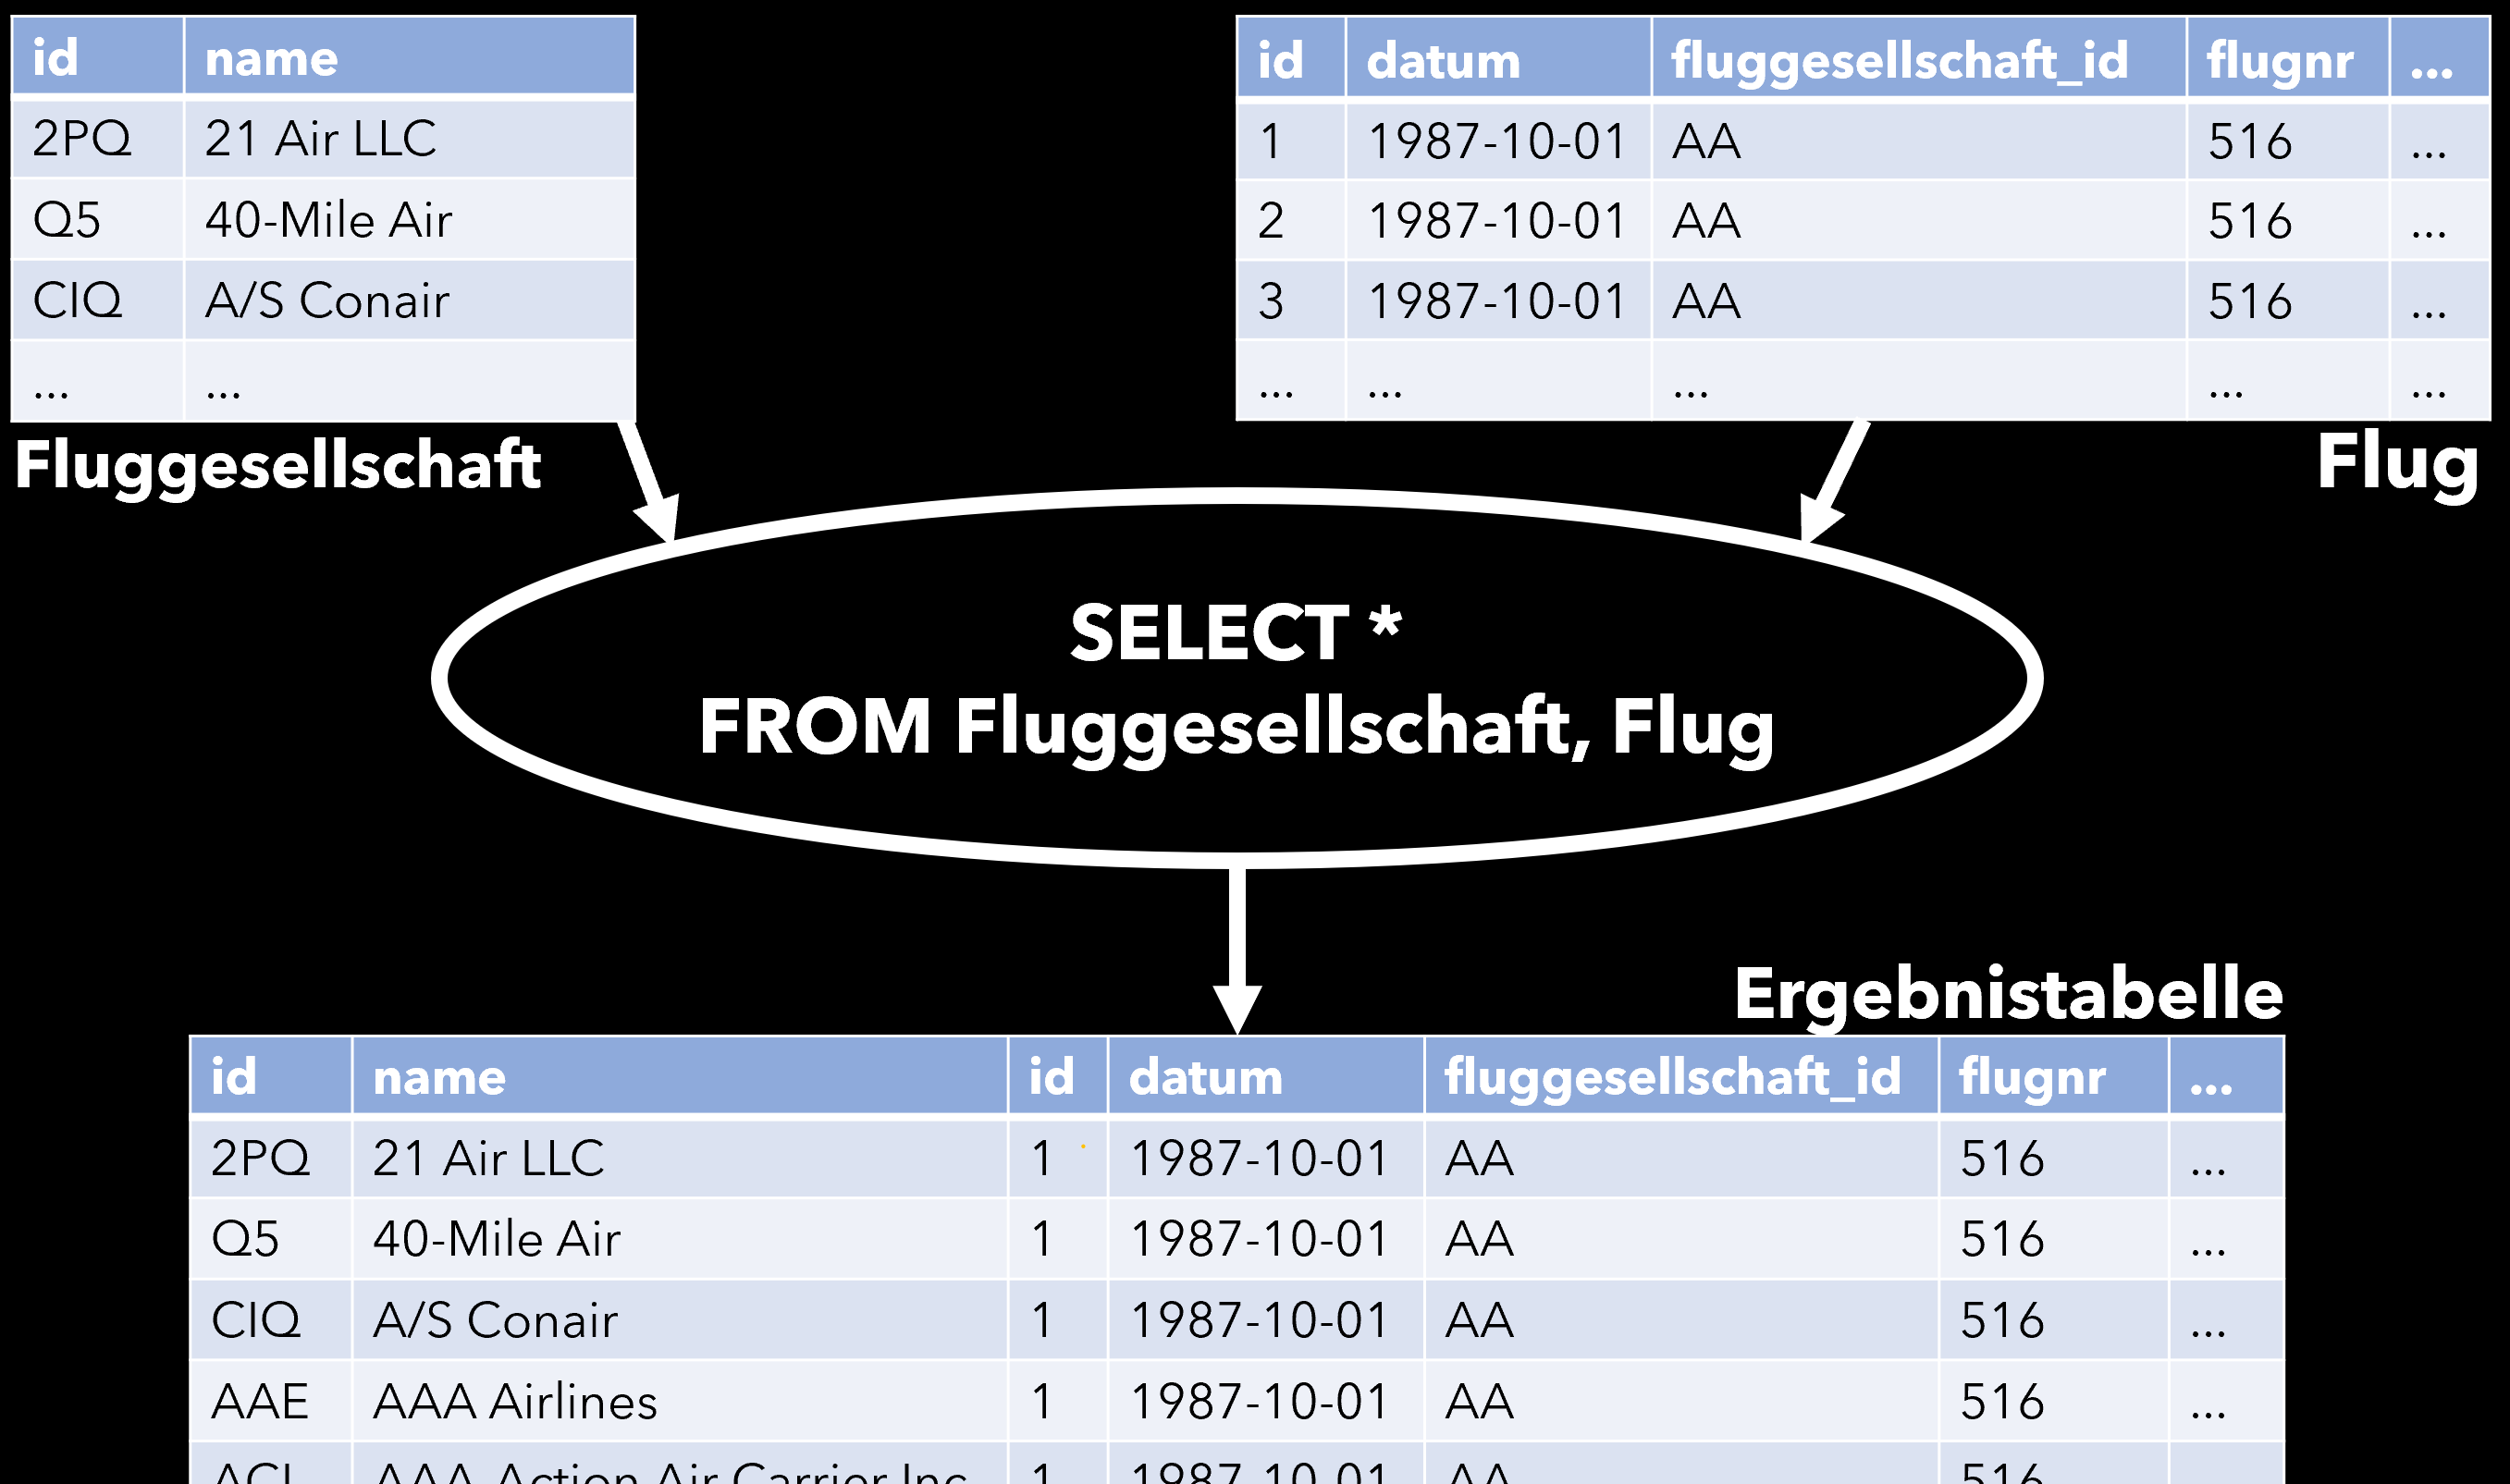
\includegraphics[height=\pageheight]{_Aufgaben/img/A07_Abfrage.png}
}
\fi

\UnterAufgabe{SQL: Tabellen verbinden}{

    Was beobachtest du? Werden nur zusammengehörende Datensätze angezeigt? Falls nicht, nach welchem Muster werden die beiden Tabellen miteinander kombiniert?

    \LoesungLine{Nein, es werden alle Datensätze aus einer mit allen Datensätzen aus der anderen kombiniert und die Spalten einfach hintereinander aufgereiht.}{3}
}